\documentclass[11pt,a4paper]{article}
\usepackage[T1]{fontenc}
\usepackage[utf8]{inputenc}
\usepackage{lmodern}
\usepackage[margin=2.5cm]{geometry}
\usepackage{amsmath,amssymb}
\usepackage{graphicx}
\usepackage{booktabs}
\usepackage{tabularx}
\usepackage[numbers,sort&compress]{natbib}
\usepackage[hidelinks]{hyperref}
\usepackage[capitalize]{cleveref}
\usepackage{caption}
\captionsetup{font=small,labelfont=bf}
\renewcommand{\bibfont}{\small}
\setlength{\bibsep}{2pt}
\renewcommand{\topfraction}{0.9}
\renewcommand{\textfraction}{0.07}
\renewcommand{\floatpagefraction}{0.8}
\renewcommand{\thesection}{S\arabic{section}}
\renewcommand{\thefigure}{S\arabic{figure}}
\renewcommand{\thetable}{S\arabic{table}}
\renewcommand{\theequation}{S\arabic{equation}}

\title{Supplementary Material for\\ ``Adaptive Time Delay Stability: Data-Driven Selection of Window Length, Lag Range and Stability Tolerance for Time-Delay Coupling Analysis''}

\author{Asaf Markuza}
\date{}

\begin{document}

\maketitle

\noindent This document holds the details referred to in the main paper as ``Supplementary Material, Section S$n$''. Notation, metrics and settings are those of the main paper (Sections 2 and 3). Fixed TDS denotes the original parameters (60 / $\pm30$ / $\pm1$ samples).

\section{Further Details of the Method}
\label{app:method}

\emph{Further test signals.} Besides the AR(1) pairs, further signal classes are fractional Gaussian noise with Hurst exponent $H$ generated by circulant embedding (long memory, $H$ equal to the DFA exponent~\cite{Peng1995QuantificationScaling}), AR(2) oscillators with period 40 and pole radius 0.97 (rhythms), two Rulkov map neurons~\cite{Rulkov2002ModelingSpikingbursting} with delayed diffusive one-way coupling (bursts), mixed-speed systems, and a record whose memory changes from $\tau_c = 4$ to 16 halfway. Records are 20\,000 samples unless stated otherwise: 30\,000 for the pair of \cref{fig:example} and the tolerance calibration figure and for the independent-sample curve of the window figure; 40\,000 for the on/off test; 6\,000 for Rulkov. The recorded test pair is the sleep-EEG $\delta$- and $\sigma$-band power pair at 1\,Hz distributed with pyTDS. The scripts underlying every figure and table, and their raw outputs, are available in the repository.

\emph{Slowest signal versus pair-specific factor.} The joint factor $B_{xy} = 1 + 2\sum_k r_x(k)\,r_y(k)$ is the tighter, pair-specific alternative to $\max_i B_i$; in the single configuration tested (\cref{fig:classes}) it yielded the same detection with a shorter window, a tighter tolerance and a lower chance score (3.9\,\% vs 5.2\,\%). The approximation of the truncated Bartlett sum fails where later negative or seasonal lobes are substantial, as in the seasonal catchment of \cref{app:seasonal}.

\emph{Computational cost.} The calibration requires at most $50 \times 20 = 1\,000$ delay series of rotated copies. Since the delay series does not depend on the tolerance, the scan over tolerances only re-applies the 4-of-5 rule to stored series; the dominant cost is therefore approximately 1\,000 sliding-window cross-correlation passes, independent of the number of tolerances evaluated.

\emph{Interpretation of scores at wide tolerance.} The calibrated tolerance increases with the time scale, but in every setting of this study it remains a small fraction of the lag range: from 4.5\,\% (rainfall--runoff, $\pm43$ of $\pm956$ samples) to 10.4\,\% ($r = 16$, $\pm56$ of $\pm541$), for example $\pm13$ of $\pm129$ in \cref{fig:example} and $\pm14$ of $\pm149$ in the capped sleep analysis. An aTDS score is therefore the fraction of windows in which the delay is stable to approximately one tenth of the lag range. Relative to the delay itself the tolerance can be large (e.g.\ $\pm13$ for a delay of 20 in the $\tau_c = 8$ simulations), but delay accuracy is assessed separately, from the $\tau_0$ of the stable windows: in the delay-pattern simulations the median error is 0 and 99\,\% of stable windows lie within 3 samples of the true delay. A wide tolerance therefore does not imply imprecise delays; it bounds the window-to-window fluctuation that is accepted.

\emph{Tolerance versus window length.} Both a longer window and a wider tolerance reduce false instability: the former reduces the jitter of $\tau_0$, the latter accommodates it. The oracle of the slow-down test (\cref{app:slowdown}) shows that, when temporal resolution is not required, long windows with tolerance 0 yield the best detection. aTDS instead fixes the window at 30 independent samples to preserve temporal resolution and uses the tolerance, bounded by the chance budget, to accommodate the remaining jitter.

\section{Illustrative Example}
\label{app:example}
\Cref{fig:example} shows one coupled pair ($\tau_c = 8$, $d = 20$, $c = 0.6$) analysed with fixed TDS and with the parameters selected by aTDS on a separate training pair of the same type ($L = 259$, $\tau_{\max} = \pm129$, $\mathrm{tol} = \pm13$). With the fixed window, $\tau_0$ is scattered and rarely remains constant for 4 of 5 windows: the TDS score is 5.2\,\%, with $\tau_0$ within $\pm2$ samples of the true delay in 28\,\% of windows. With aTDS, $\tau_0$ coincides with the true delay: the score is 91.3\,\%, with $\tau_0$ within $\pm2$ samples in 90\,\% of windows. The coupling is identical in both cases; only the parameters differ. For the unrotated pair the score at tolerance 0 is 90.0\,\% and at $\pm13$ 91.3\,\%.

\begin{figure}[!htbp]
\centering
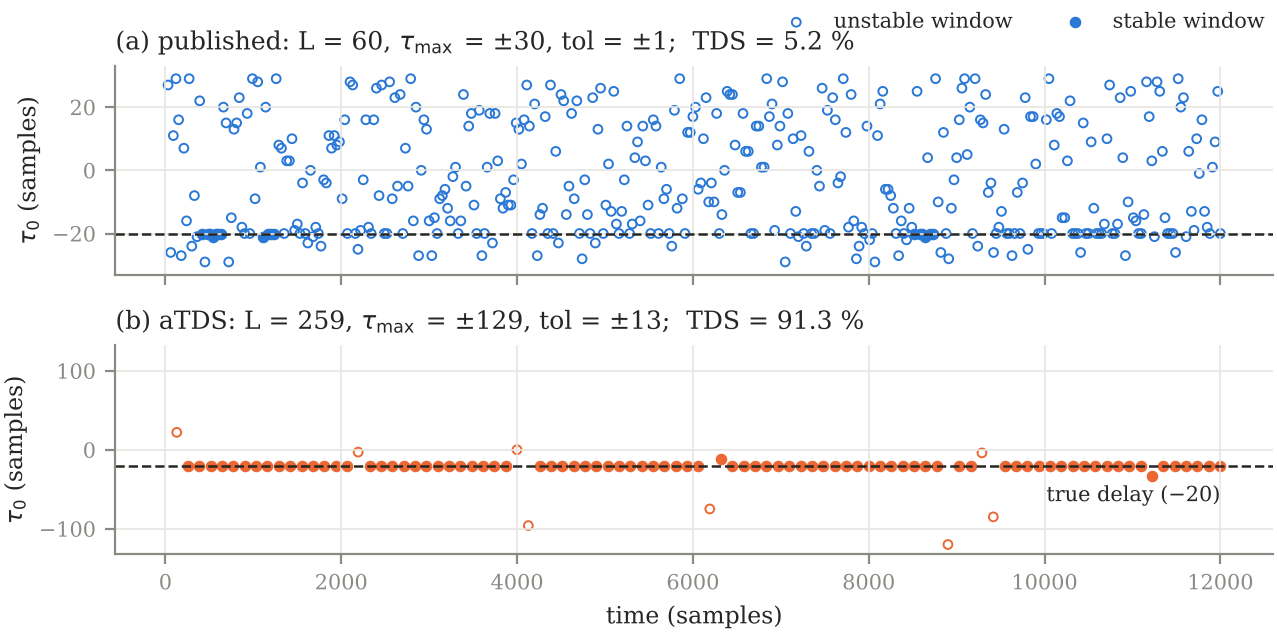
\includegraphics[width=0.85\textwidth]{figures/fig_example_fixed_vs_atds.png}
\caption{The same coupled pair ($\tau_c = 8$, true delay 20 samples, coupling 0.6) under fixed parameters (a) and the parameters chosen by aTDS on a separate training pair (b). Each dot is $\tau_0$ in one window over the first 12\,000 samples; filled dots are stable windows. The dashed line is the true delay of 20 samples, plotted as $\tau_0 = -20$ ($x$ leads).}
\label{fig:example}
\end{figure}

\section{Further Evaluation of the Rules}
\label{app:rules}
\subsection{Window Constant under Intermittent Coupling}
\label{app:onoff}
To evaluate the constant 30 when temporal resolution is relevant, coupling ($c = 0.6$, $\tau_c = 8$, $d = 20$) was switched on and off in blocks of 1\,000, 2\,000 or 4\,000 samples (40\,000 samples, 20 pairs per point). A window was counted as correct if it was stable with $\tau_0$ within $\pm2$ samples of the true delay during coupling, or not stable in the absence of coupling. \Cref{fig:onoff} shows a genuine trade-off whose optimum depends on episode length: 45 independent samples for the shortest blocks (balanced accuracy 0.87, compared with 0.85 at 30), 60 for 2\,000-sample blocks (0.92, compared with 0.88 at 30), and a plateau of 0.94--0.95 from 45 onwards for the longest blocks (0.91 at 30). In all three cases the aTDS constant lies within 0.015--0.05 of the optimum, on the side of shorter windows.

\begin{figure}[!htbp]
\centering
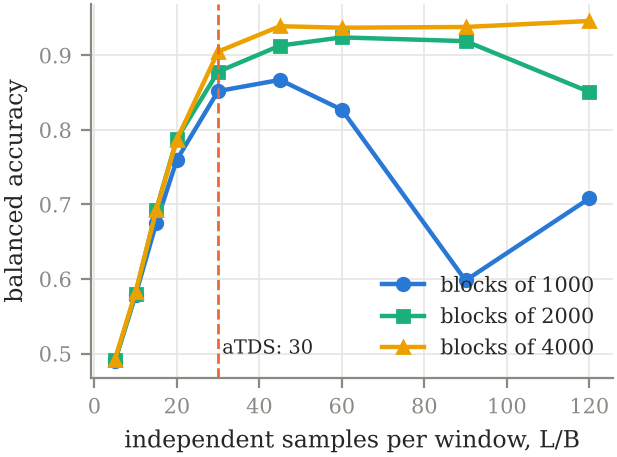
\includegraphics[width=0.5\textwidth]{figures/fig_onoff_tradeoff.png}
\caption{Coupling switched on and off in blocks of 1\,000--4\,000 samples. Balanced accuracy of the window labels against the number of independent samples per window; dashed line: the aTDS constant 30.}
\label{fig:onoff}
\end{figure}

\subsection{Tolerance Rule: Stable Windows}
\label{app:tolerance}
In the tolerance-only comparison of the main paper (evaluation of the tolerance rule), the improvement in delay recovery results from a sufficient number of stable windows: with $\pm1$, only 77, 66 and 26 of 100 coupled pairs at $r = 4, 8, 16$ have 3 or more stable windows (nearly all of them correct), whereas with calibration 98, 93 and 53 pairs do, of which 90, 91 and 79\,\% are correct.

\subsection{Sensitivity to the Design Constants}
\label{app:sens}
Beyond the constant 30, the design constants were varied one at a time in the slow-down test ($r = 1$, 4, 8; 100 + 100 pairs per $r$), all others at their defaults (\cref{tab:sensitivity}). The AUC changes by at most about 0.05 for the budget, the SE multiplier, the minimum window and the number of rotations. The number of independent samples per window trades detection against temporal resolution: larger values detect better at slow time scales, as the oracle shows, at the cost of fewer and longer windows (\cref{fig:onoff}). The rhythm threshold decides whether the half-period cap is applied: in the rhythm case (period about 40), thresholds 0.2 and 0.3 detect the rhythm, cap the lag at $\pm20$ and find the delay in 100\,\% of pairs at $d = 8$ and 0\,\% at $d = 30$ (AUC 1.00 / 0.995); at 0.4 the rhythm is not detected, the lag range is not capped (lag $\pm157$, tolerance $\pm16$), and the delay of 30 is found in 100\,\% of pairs, as is the delay of 8 (AUC 1.00 / 1.00). In this test the default cap is therefore worse for the delay beyond half a period. The cap trades lag range for an unambiguous delay within half a period: for a periodic signal, delays $d$ and $d - P$ beyond half a period are ambiguous for any windowed cross-correlation; the AR(2) rhythm of this test is only approximately periodic, and there an uncapped range can find a delay beyond half a period. The 50-pair cap and the rotation exclusion zone $a$ were not varied.

\begin{table}[!htbp]
\centering
\caption{Sensitivity of aTDS to its design constants in the slow-down test (100 coupled and 100 uncoupled pairs per $r$), one constant varied at a time; defaults in bold. Tolerance: calibrated tolerance at $r = 1$ / 4 / 8 (samples), given where it differs from the default.}
\label{tab:sensitivity}
\footnotesize
\begin{tabular}{llcccc}
\toprule
Constant & Value & AUC, $r = 1$ & $r = 4$ & $r = 8$ & Tolerance \\
\midrule
All constants at default & & 0.995 & 0.923 & 0.877 & 3 / 12 / 27 \\
\midrule
Independent samples per window & 15 & 0.997 & 0.717 & 0.684 & \\
\quad (default \textbf{30}) & 45 & 1.000 & 0.946 & 0.899 & \\
 & 60 & 1.000 & 0.991 & 0.954 & \\
False-stability budget & 1\,\% & 1.000 & 0.920 & 0.884 & 1 / 4 / 9 \\
\quad (default \textbf{5\,\%}) & 10\,\% & 0.981 & 0.874 & 0.851 & 4 / 18 / 40 \\
SE multiplier $z$ (default \textbf{2}) & 0 & 0.995 & 0.911 & 0.861 & \\
 & 3 & 0.995 & 0.923 & 0.881 & \\
Minimum window $L_{\min}$ (default \textbf{61}) & 31 & 0.995 & 0.923 & 0.877 & \\
 & 121 & 1.000 & 0.923 & 0.877 & \\
Rotations per pair (default \textbf{20}) & 10 & 0.995 & 0.921 & 0.888 & \\
 & 40 & 0.995 & 0.923 & 0.862 & \\
\bottomrule
\end{tabular}
\end{table}

\section{Slow-Down Test: All Settings}
\label{app:slowdown}
\Cref{tab:slowdownfull} lists the AUC of all four settings of the slow-down test, including the manually rescaled setting (given the true $r$) and the oracle, with the parameters chosen by aTDS and the oracle. At $r = 4$ the AUC of aTDS is 0.92 vs 0.59 for fixed TDS. The manually rescaled setting is marginally higher than aTDS at $r = 2$ (0.99 vs 0.98), and aTDS is better than it at $r = 8$ (0.88 vs 0.81; delay found in 85\,\% vs 60\,\% of pairs). In the comparison with rescaled fixed TDS (main paper, Table 2), rescaled fixed TDS is slightly higher at $r = 2$ and 4 (AUC 0.993 vs 0.979 and 0.955 vs 0.923), aTDS is higher at $r = 8$ (0.877 vs 0.806), and at $r = 16$ the AUC of aTDS is 0.65 with a paired difference to fixed TDS of $+0.14$ [0.03, 0.25].

\begin{table}[!htbp]
\centering
\caption{Slow-down test: AUC [95\,\% interval] of all settings and parameters chosen. Window / lag / tolerance in samples.}
\label{tab:slowdownfull}
\resizebox{\textwidth}{!}{%
\begin{tabular}{rcccccc}
\toprule
$r$ & Fixed TDS & Manually rescaled (true $r$) & aTDS & Oracle & aTDS parameters & Oracle parameters \\
\midrule
1  & 0.997 [0.989, 1.00] & 0.997 [0.989, 1.00] & 0.995 [0.988, 1.00] & 1.000 [0.999, 1.00] & 66 / 32 / 3     & 60 / 29 / 0 \\
2  & 0.888 [0.839, 0.93] & 0.993 [0.984, 1.00] & 0.979 [0.961, 0.99] & 1.000 [1.00, 1.00] & 126 / 62 / 6    & 240 / 119 / 0 \\
4  & 0.590 [0.513, 0.66] & 0.955 [0.926, 0.98] & 0.923 [0.885, 0.96] & 1.000 [1.00, 1.00] & 237 / 118 / 12  & 960 / 479 / 0 \\
8  & 0.541 [0.464, 0.62] & 0.806 [0.752, 0.86] & 0.877 [0.829, 0.92] & 0.985 [0.965, 1.00] & 563 / 281 / 27  & 1920 / 959 / 0 \\
16 & 0.509 [0.428, 0.59] & 0.688 [0.631, 0.74] & 0.645 [0.580, 0.72] & 0.843 [0.788, 0.89] & 1083 / 541 / 56 & 1920 / 959 / 135 \\
\bottomrule
\end{tabular}}
\end{table}

\section{Further Signal Classes}
\label{app:classes}
\Cref{fig:classes} compares aTDS with fixed TDS on signal classes characteristic of physiology; in every case aTDS set its parameters on data that were not scored. aTDS performs better for signals with strong long memory ($H = 0.9$), rhythms with delays below half a period, changing dynamics and Rulkov neurons, and equally or indistinguishably for $H = 0.6$ and 0.75. For a rhythm with a delay beyond half a period, the coupling is detected but the delay is incorrect, as expected from the lag cap. For a fast signal with a long delay (50 samples), the default lag range ($\pm30$) is too short and the optional $d_{\max}$ is required; without it the delay is missed by both settings (AUC 0.56).

Two cases indicate possible refinements. In a mixed-speed system, a single window determined by the slowest signal assigns a wide tolerance to fast pairs ($\pm56$ instead of $\pm3$ with a per-pair window). For a coupled fast--slow pair, the joint Bartlett factor $B_{xy}$ (11.3, between $B_x = 31.3$ and $B_y = 5.0$) yielded the same detection with a window 2.8 times shorter and a tolerance 2.7 times tighter than the max-$B$ rule. For Rulkov neurons, the delay was reported a constant 3 steps too long at both delays, presumably reflecting the response latency of the map; calibration did not fail under one-way coupling. The AUC values of all classes are listed in \cref{tab:scoreboard}.

\begin{figure}[!htbp]
\centering
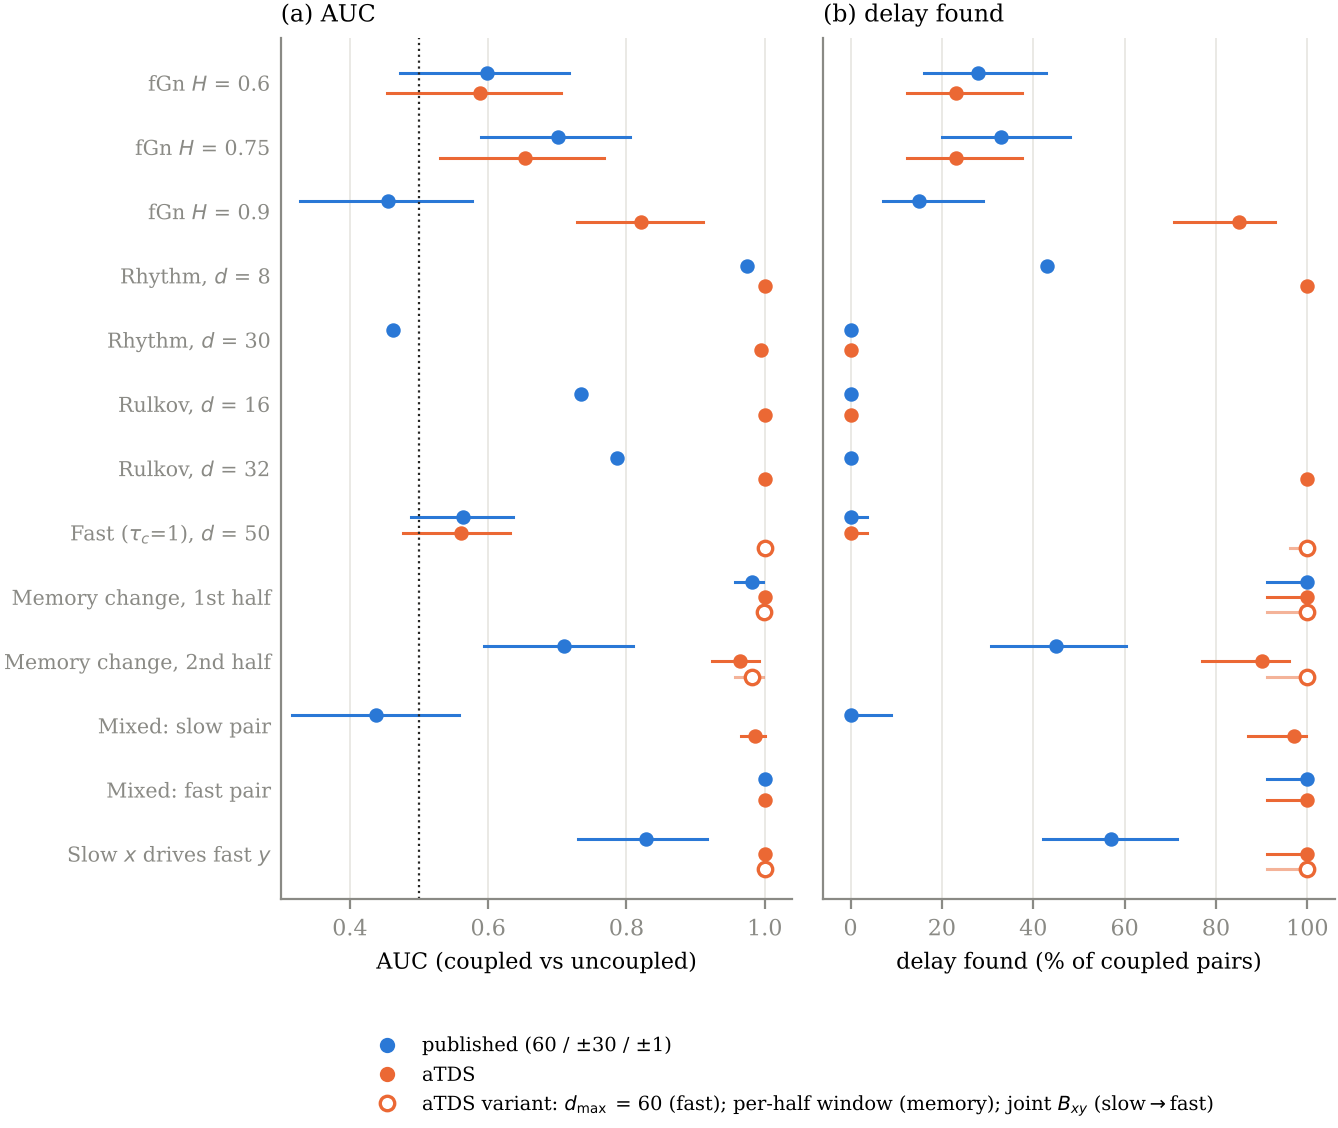
\includegraphics[width=0.8\textwidth]{figures/fig_signal_classes.png}
\caption{Other signal classes. (a) AUC, coupled vs uncoupled pairs, with bootstrap 95\,\% intervals where available; dotted: chance. (b) Share of coupled pairs whose stable windows report the true delay, with Wilson 95\,\% intervals. Hollow markers: aTDS variants (optional $d_{\max} = 60$ for the fast signal; one window per half for the memory change; joint Bartlett factor for the slow--fast pair). For Rulkov neurons ``delay found'' uses the strict rule: aTDS reports the delay a constant 3 steps too long (19 and 35), so it counts as found only at $d = 32$ within the tolerance of the rule; its AUC is 1.0 at both delays.}
\label{fig:classes}
\end{figure}

\section{Physiological Recordings: EEG Pair, ECG Details and Delay Reference}
\label{app:physio}
\Cref{fig:physiotraces} shows the delay found in every window for two physiological pairs with known delays: sleep EEG power at 1\,Hz (delay 0) and ECG and finger pulse at 125\,Hz. A coupled pair appears as a horizontal line of stable windows at the true delay.

\begin{figure}[!htbp]
\centering
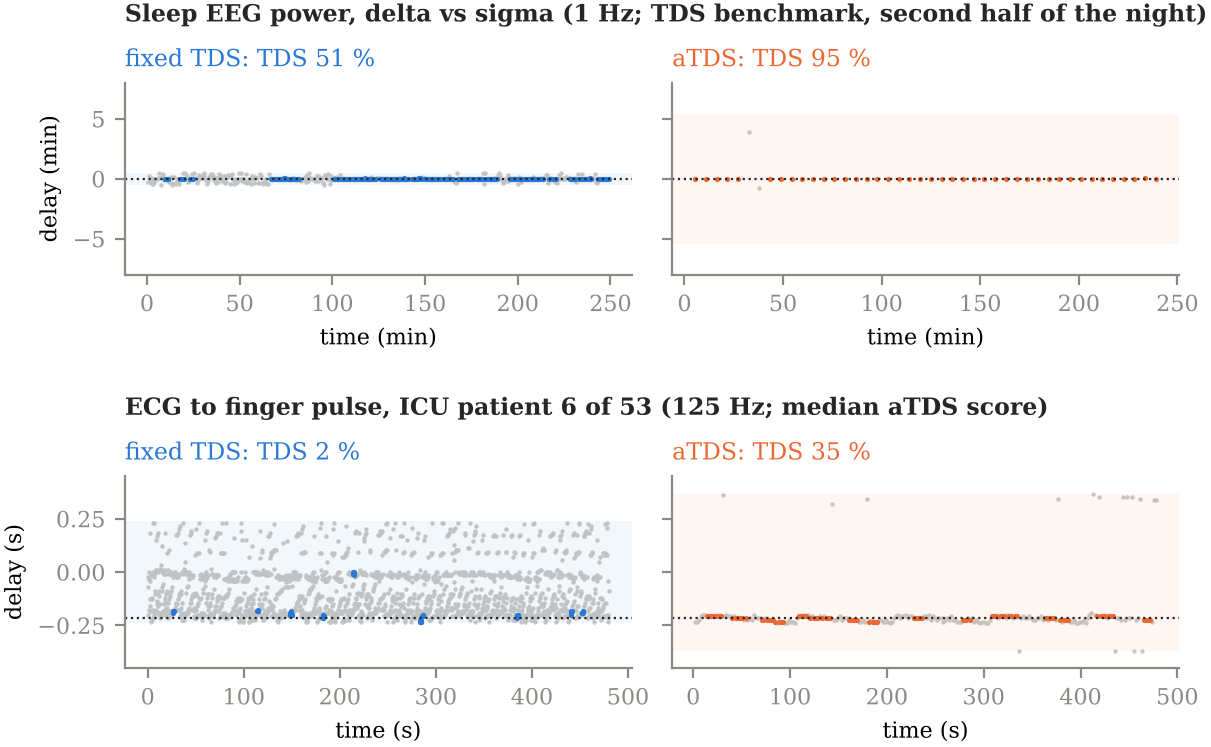
\includegraphics[width=0.8\textwidth]{figures/fig_physio_traces.png}
\caption{$\tau_0$ in each window (the reported delay is $-\tau_0$), fixed TDS (left) and aTDS (right). Coloured: stable windows; grey: unstable windows; shaded band: the lag range searched; dotted line: the reference delay (0 for the EEG pair; the full-record alignment of the two waveforms for the ECG pair). EEG: parameters set on the first half of the night and scored on the second. ECG: the patient with the median aTDS score among the 53. For the EEG pair both settings recover the delay; for the ECG pair only aTDS yields a continuous line of stable windows at the reference delay.}
\label{fig:physiotraces}
\end{figure}

\paragraph{Benchmark sleep-EEG pair.} With parameters set on the first half of the night and scores computed on the second half, fixed TDS scores 50.8\,\% against a chance level of 1.2\,\% (95th percentile 2.6\,\%), and aTDS (window 652\,s, lag $\pm325$\,s, tolerance $\pm22$\,s) 95.5\,\% against 2.1\,\% (95th percentile 11.4\,\%); capped at 300\,s, aTDS scores 82.7\,\% against 2.3\,\%. Both are significant at the smallest $p$ attainable with 100 rotations ($p \le 0.01$). Since no ground truth beyond detection is available, this pair does not permit a ranking of the two settings.

\paragraph{ECG with per-pair aTDS parameters.} At 125\,Hz the fixed window of 60 samples spans 0.48\,s, less than one heartbeat, and its lag range of $\pm0.24$\,s covers less than half a beat. Fixed TDS detected the coupling in few patients: median score 1.6\,\% (control mean 1.2\,\%), 14 of 53 patients above the 95th percentile of the controls, AUC 0.69 (95\,\% interval 0.58--0.79). With parameters set separately for each pair, aTDS selected windows of 2.9--5.9\,s (median 4.3\,s, six to seven heartbeats) and a lag range of approximately half a heartbeat (median $\pm0.34$\,s, determined by the rhythm cap). It detected the coupling in 49 of 53 patients (median score 35\,\%; AUC 0.95, 0.90--0.99) and yielded a higher score than fixed TDS in 47 of 53 (\cref{tab:bidmcpair}). The mean aTDS score of the controls was 3.3\,\% (95th percentile 7.5\,\%). In 12 of the 53 true pairs, the tolerance calibration could not satisfy the 5\,\% budget even at zero tolerance, because rotated copies of a heartbeat signal remain aligned with the ECG by chance; these pairs were scored with tolerance 0. Because per-pair parameters score true pairs and controls on different scales and depend on per-pair calibration, the main paper reports one parameter set for all 106 pairs ($L = 539$ samples, 4.31\,s). With it, true pairs scored a mean of 28.5\,\% (median 25.2\,\%) and controls 0.25\,\% (95th percentile 1.26\,\%), AUC 0.96 (0.93--0.99), with 50 of 53 patients above the controls' 95th percentile. Rescaled fixed TDS (window 480 samples, lag range $\pm240$ samples, three median heartbeats of 0.64\,s) scored a mean of 59.9\,\% (median 63.1\,\%) in true pairs; its AUC equalled that of aTDS (0.962 vs 0.963), but its controls' 95th percentile was 39\,\% instead of 1.3\,\%, so that 43 rather than 50 of 53 patients exceeded it.

\begin{table}[!htbp]
\centering
\caption{ECG and finger pulse at 125\,Hz, 53 intensive-care patients (BIDMC). aTDS: parameters per pair, except the row ``one set for all pairs'' ($L = 4.31$\,s, $\pm0.34$\,s, tolerance 0; fixed TDS is a single set by construction). Delay agreement is modulo one heartbeat.}
\label{tab:bidmcpair}
\footnotesize
\begin{tabular}{lcc}
\toprule
 & Fixed TDS & aTDS \\
\midrule
Window / lag range / tolerance & 0.48\,s / $\pm0.24$\,s / $\pm8$\,ms & 2.9--5.9\,s / $\approx\pm0.34$\,s / mostly 0 \\
Median score, true pairs & 1.6\,\% & \textbf{35\,\%} \\
Mean score, controls (95th percentile) & 1.2\,\% (5.7\,\%) & 3.3\,\% (7.5\,\%) \\
AUC, true pairs vs controls [95\,\% interval] & 0.69 [0.58, 0.79] & \textbf{0.95} [0.90, 0.99] \\
Patients above the controls' 95th percentile & 14 / 53 & \textbf{49 / 53} \\
One set for all pairs: AUC; patients above & 0.69; 14 / 53 & \textbf{0.96} [0.93, 0.99]; \textbf{50 / 53} \\
Patients with the higher score & 6 / 53 & \textbf{47 / 53} \\
Patients with a delay (3+ stable windows) & 41 / 53 & 53 / 53 \\
Delay within 0.1\,s of pulse arrival time & \textbf{32 / 41} & 24 / 53 \\
Delay within 0.04\,s of full-record alignment & 22 / 41 & \textbf{40 / 53} \\
\bottomrule
\end{tabular}
\end{table}

\paragraph{ECG delay reference.}
\label{app:ecgdelay}
Because the heartbeat is periodic, a delay between the ECG and pulse waveforms is defined only up to one beat, and TDS, which uses the absolute correlation, may also lock onto a lag half a beat away. The reference delay of each patient is taken as the alignment of the two waveforms over the entire 8-minute record (the peak of the full-record cross-correlation within half a beat), which is independent of any window setting. aTDS with per-pair parameters reported a delay in all 53 patients and agreed with this reference within 0.04\,s in 40 of them; fixed TDS reported a delay in 41 patients (3 or more stable windows) and agreed with it in 22 (\cref{fig:bidmcdelay}). With one parameter set for all pairs, aTDS reported a delay in 50 patients, within 0.04\,s of the full-record alignment in 38 of them (median difference 0.000\,s); rescaled fixed TDS reported a delay in all 53 patients, within 0.04\,s of the full-record alignment (modulo one beat) in 41. The pulse arrival time measured beat by beat, from the ECG R peak to the steepest point of the pulse upstroke, constitutes a different reference, as it marks a single point of the pulse wave rather than the entire waveform. Relative to this reference, aTDS was within 0.1\,s (modulo one beat) in 24 of 53 patients (median difference 0.07\,s), and fixed TDS, whose short window aligns the sharp ECG spike with the pulse upstroke, in 32 of its 41.

\begin{figure}[!htbp]
\centering
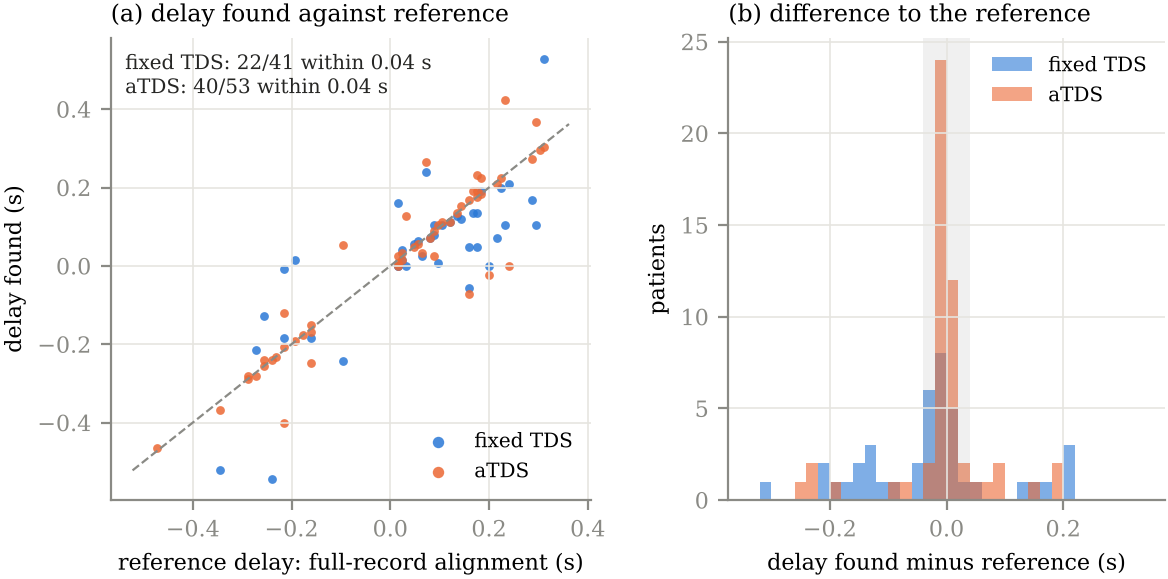
\includegraphics[width=0.75\textwidth]{figures/fig_bidmc_delay.png}
\caption{ECG to finger pulse, 53 patients: (a) delay found per patient against the reference delay (full-record alignment of the two waveforms), fixed TDS (blue, 41 patients with a delay) and aTDS (orange, 53); found delays are shown modulo one heartbeat around the reference. (b) Distribution of the difference.}
\label{fig:bidmcdelay}
\end{figure}

\subsection*{Ablation: aTDS rules added to rescaled fixed TDS}
All settings use one parameter set for the 106 pairs. Rhythm cap: the lag range of the common aTDS set ($\pm42$ samples). Calibrated tolerance: the aTDS tolerance rule applied to the given window and lag range.

\begin{table}[h]
\centering
\caption{ECG and finger pulse, 53 patients: rescaled fixed TDS ($\hat r = 8$) with the aTDS rules added one at a time.}
\footnotesize
\begin{tabular}{lccccc}
\toprule
Setting & $L$ / $\tau_{\max}$ / tol & AUC & Controls mean (95th pct) & Above controls & \\
\midrule
Rescaled fixed TDS & 480 / $\pm240$ / $\pm8$ & 0.962 & 6.8\,\% (39.2\,\%) & 43 / 53 & \\
+ calibrated tolerance & 480 / $\pm240$ / 0 & 0.928 & 0.10\,\% (0.0\,\%) & 46 / 53 & \\
+ rhythm cap & 480 / $\pm42$ / $\pm8$ & 0.973 & 20.6\,\% (60.0\,\%) & 48 / 53 & \\
+ both & 480 / $\pm42$ / 0 & 0.945 & 0.26\,\% (1.6\,\%) & 46 / 53 & \\
aTDS & 539 / $\pm42$ / 0 & 0.963 & 0.25\,\% (1.26\,\%) & 50 / 53 & \\
\bottomrule
\end{tabular}
\end{table}

\subsection*{Held-out halves}
Patients were split at random (seed 0) into halves of 26 and 27. Parameters set on one half (aTDS: $L$ = 537 and 543, $\tau_{\max} = \pm41$ and $\pm42$, tolerance 0; rescaled fixed TDS: $\hat r$ = 7 and 8) were applied to the other half, whose controls pair the ECG of each patient with the pulse of the next patient of the same half. AUC [95\,\% interval], test half of 27 / 26: fixed TDS 0.648 [0.487, 0.800] / 0.746 [0.603, 0.878]; rescaled fixed TDS 0.968 [0.926, 0.996] / 0.994 [0.978, 1.0]; aTDS 0.980 [0.936, 1.0] / 0.976 [0.932, 1.0].

\section{Sleep Cohort: Design, Stage Contrasts and Stage-Aware Selection}
\label{app:cohort}
\paragraph{Data and design.} We analysed 35 overnight polysomnographic recordings prepared in the author's MSc project to reproduce the network analysis of Bashan et al.~\cite{Bashan2012NetworkPhysiology}. Each recording has 10 channels at 1\,Hz: heart rate, respiratory rate, the standard deviation of chin EMG, leg EMG and EOG, and the $\delta$, $\theta$, $\alpha$, $\sigma$ and $\beta$ EEG band powers; recordings last 23\,150--31\,752\,s and are scored into wake (W), light sleep (LS), deep sleep (DS) and REM. The cohort analysis uses the default, non-causal stability anchor. We compared three settings, each a single parameter set for the whole cohort: fixed TDS; aTDS, with the window from the median over subjects of $\max_i B_i$ (228) and the tolerance calibrated on rotations pooled over 50 random subject--pair combinations, giving $L = 2\,868$\,s (the 10\,\% cap), $\tau_{\max} = \pm1\,433$\,s and $\mathrm{tol} = \pm136$\,s; and aTDS with the window capped at 300\,s ($\tau_{\max} = \pm149$\,s, $\mathrm{tol} = \pm14$\,s). For each subject, each of the 45 links and each setting, the delay series and stability labels were computed over the whole night; a window was assigned to a stage if at least 80\,\% of its seconds carried that stage, and the per-stage TDS is the percentage of stable windows among those assigned (at least 3 required). Significance used the cross-subject, stage-matched null of the original studies~\cite{Bashan2012NetworkPhysiology}: for each link, 100 surrogate pairs combined channel $i$ of one subject with channel $j$ of another, scored with the first subject's stages, and a link was significant in a subject and stage if its TDS exceeded the 95th percentile of this null.

\paragraph{Temporal resolution of the uncapped window.} With a 48-minute window, no subject had three windows lying at least 80\,\% within wake, REM or deep sleep, and only 24 subjects had three in light sleep; in this cohort the uncapped setting therefore cannot resolve sleep stages, because the window required by the slowest signals is far longer than a typical stage episode (median 300\,s), and stage-resolved analyses of these data must impose a cap.

\paragraph{Sleep-stage contrasts.} \Cref{tab:cohort} compares fixed TDS with aTDS capped at 300\,s. Raw scores are higher under aTDS in every stage because of its wider tolerance and are therefore not comparable across settings; the number of links that are significant against the stage-matched null provides the appropriate comparison. Both settings show the strong light- versus deep-sleep contrast: mean link TDS, $d_z = 1.37$ (fixed TDS) and 1.65 (aTDS), with light sleep higher in 91\,\% and 94\,\% of subjects; the gain, $+0.31$ (95\,\% interval $-0.06$ to $+0.75$), is not significant, and for significant links the gain is not significant either ($-0.14$, $-0.74$ to $0.47$). Under fixed TDS REM had lower mean link TDS than deep sleep ($d_z = -0.50$, interval $-0.88$ to $-0.17$), although it had more significant links ($d_z = 0.75$); under aTDS the mean-TDS inversion disappeared ($d_z = 0.11$, $-0.25$ to $0.42$; gain $+0.67$, $0.40$ to $0.98$), and the significant-link contrast was unchanged (gain $+0.15$, $-0.20$ to $0.50$). The wake contrast was weaker under aTDS ($d_z = 0.29$ vs 0.57 for mean TDS; for significant links, gain $-1.17$, $-1.65$ to $-0.77$) and is based on only 26 subjects: 8 subjects lack three pure 300-s wake windows and one lacks deep-sleep windows. No ground truth exists for the REM ordering: the change in mean TDS may reflect the wider tolerance rather than physiology, and the significant-link contrast, which is calibrated against the null of each setting, did not change. This change is therefore not regarded as an improvement. On recorded, sleep-staged data, aTDS does not sharpen sleep-stage contrasts: it reproduces the principal contrast, leaves the significant-link contrasts unchanged or weaker, and loses statistical power where stage episodes are short. Wake episodes (median 90\,s) are short relative to the window that these slow signals require; this loss of power is a property of these data rather than of the rule.

\begin{table}[!htbp]
\centering
\caption{Sleep-stage contrasts in 35 subjects: paired effect size $d_z$ [95\,\% bootstrap interval] and share of subjects with a positive difference. Gain: aTDS (300\,s cap) minus fixed TDS, paired. $n$ = subjects with enough stage windows (fixed TDS: 35).}
\label{tab:cohort}
\footnotesize
\resizebox{\textwidth}{!}{%
\begin{tabular}{llccc}
\toprule
Measure & Contrast & Fixed TDS & aTDS, 300\,s cap ($n$) & Gain \\
\midrule
Mean link TDS & LS $-$ DS & 1.37 [1.02, 1.91] (91\,\%) & 1.65 [1.27, 2.25] (94\,\%) (34) & $+0.31$ [$-0.06$, 0.75] \\
 & W $-$ DS & 0.57 [0.25, 0.97] (69\,\%) & 0.29 [$-0.09$, 0.76] (65\,\%) (26) & $-0.28$ [$-0.70$, 0.13] \\
 & REM $-$ DS & $-0.50$ [$-0.88$, $-0.17$] (40\,\%) & 0.11 [$-0.25$, 0.42] (47\,\%) (34) & $+0.67$ [0.40, 0.98] \\
 & LS $-$ REM & 1.90 [1.53, 2.53] (100\,\%) & 1.37 [0.97, 1.97] (91\,\%) (35) & $-0.53$ [$-1.18$, 0.05] \\
\midrule
Significant links & LS $-$ DS & 2.58 [2.11, 3.41] (100\,\%) & 2.47 [1.95, 3.34] (100\,\%) (34) & $-0.14$ [$-0.74$, 0.47] \\
 & W $-$ DS & 1.16 [0.69, 1.88] (89\,\%) & 0.34 [$-0.04$, 0.95] (69\,\%) (26) & $-1.17$ [$-1.65$, $-0.77$] \\
 & REM $-$ DS & 0.75 [0.45, 1.13] (74\,\%) & 0.88 [0.58, 1.25] (74\,\%) (34) & $+0.15$ [$-0.20$, 0.50] \\
 & LS $-$ REM & 1.67 [1.26, 2.40] (94\,\%) & 1.75 [1.35, 2.39] (94\,\%) (35) & $+0.08$ [$-0.48$, 0.54] \\
\bottomrule
\end{tabular}}
\end{table}

\paragraph{Stage-aware parameter selection.}
\label{sec:res-stage}
The 300-s cap above was chosen by the analyst, and the tolerance was calibrated on rotations that ignore the stage structure. Both were therefore also derived from the sleep stages. Stage episodes had a median length of 300\,s over all stages (wake 90\,s, light sleep 420\,s, deep sleep 480\,s, REM 480\,s; 1\,573 episodes). The stage-aware setting used half the median episode length as window, $L = 150$\,s ($\tau_{\max} = \pm74$\,s), and calibrated a tolerance \emph{per stage} on 50 cross-subject, stage-matched surrogates with the same rule (mean + 2 SE $\le 5$\,\%), giving $\pm6$\,s for wake, light and deep sleep and $\pm4$\,s for REM. With this setting 33 subjects contributed to the wake contrast (26 with the 300-s cap). All contrasts kept the signs of fixed TDS: mean link TDS $d_z = 1.62$ (light vs deep), 0.53 (wake vs deep), $-0.70$ (REM vs deep) and 2.16 (light vs REM). None of the gains over fixed TDS was significant (mean link TDS: $+0.28$, interval $-0.01$ to $0.57$, for light vs deep; $+0.26$, $-0.21$ to $0.88$, for light vs REM), and in significant links the wake contrast was again weaker ($-1.02$, $-1.48$ to $-0.68$). Stage-aware calibration thus removes the arbitrary cap and the rotation null from the sleep analysis without altering its conclusion: on 1-Hz sleep networks, the regime for which the fixed parameters were chosen, aTDS does not improve upon them.

\section{Records from Other Fields: Parameters and Seasonal Catchment}
\label{app:seasonal}
\Cref{tab:fieldsfull} gives the aTDS parameters for every record and the capped analysis of the seasonal catchment, and \cref{fig:fieldssummary} compares the delay found with the expected delay. The recovered delays are 8\,h from rainfall to river flow in the hourly catchment, 2 days in the daily catchment L0123001 (expected 0--3 days), and 1\,h from temperature to electricity demand. For crude oil and gasoline, aTDS detects strong coupling (92.5\,\%, $p = 0.005$) but reports no delay.

\paragraph{Seasonal catchment L0123002.} For L0123002, the aTDS score is not significant ($p = 0.10$) and the reported delay is 162 days. The river flow of this catchment is strongly seasonal (autocorrelation 0.62 at a lag of one year); the first-zero Bartlett factor of the flow (38.8) ignores the seasonal lobe and yields a window of approximately three years with only 19 windows, of which 4 were stable. No domain value is available for the delay of this catchment; the full-record cross-correlation has its positive peak at +1 day ($r = 0.054$; the absolute peak lies at the boundary of the search). Capping the window at 120 days recovered this 1-day delay (score 10.3\,\% vs a 95th percentile of 7.4\,\%, $p = 0.015$), whereas a cap at 365 days did not (no stable window). Seasonal signals, like rhythmic signals, therefore require a window cap below the seasonal period.

\begin{table}[!htbp]
\centering
\caption{aTDS on records from other fields, with parameters. Score vs the 95th percentile of 200 rotated copies (null95); delay found = $-\tau_0$, with $\tau_0$ the most frequent value among stable windows, positive when the driver (rain, temperature, crude oil) leads.}
\label{tab:fieldsfull}
\footnotesize
\resizebox{\textwidth}{!}{%
\begin{tabular}{llcccc}
\toprule
Record & Expected delay & aTDS parameters ($L$ / $\tau_{\max}$ / tol) & Score (null95) & $p$ & Delay found \\
\midrule
Rainfall $\to$ river flow, hourly (L0123003) & about 8\,h & 79.8\,d / 39.8\,d / 1.8\,d & 79.5\,\% (9.1) & 0.005 & \textbf{8\,h} \\
Rainfall $\to$ river flow, daily (L0123001) & 0--3 days & 501 / 250 / 20 days & 97.6\,\% (12.3) & 0.005 & \textbf{2 days} \\
Rainfall $\to$ river flow, daily (L0123002) & 1 day (positive xcorr peak) & 1\,059 / 367 / 9 days & 21.1\,\% (21.1) & 0.10 & 162 days (not resolved) \\
\quad window capped at 120 days & & & 10.3\,\% (7.4) & 0.015 & 1 day \\
Temperature $\to$ electricity demand & about 1\,h & 27.1\,d / 13.5\,d / 1.0\,d & 100\,\% (21.1) & 0.005 & \textbf{1\,h} \\
Crude oil $\to$ gasoline, weekly changes & 1--2 weeks & 64 / 31 / 3 weeks & 92.5\,\% (15.1) & 0.005 & 0 weeks \\
\bottomrule
\end{tabular}}
\end{table}

\begin{figure}[!htbp]
\centering
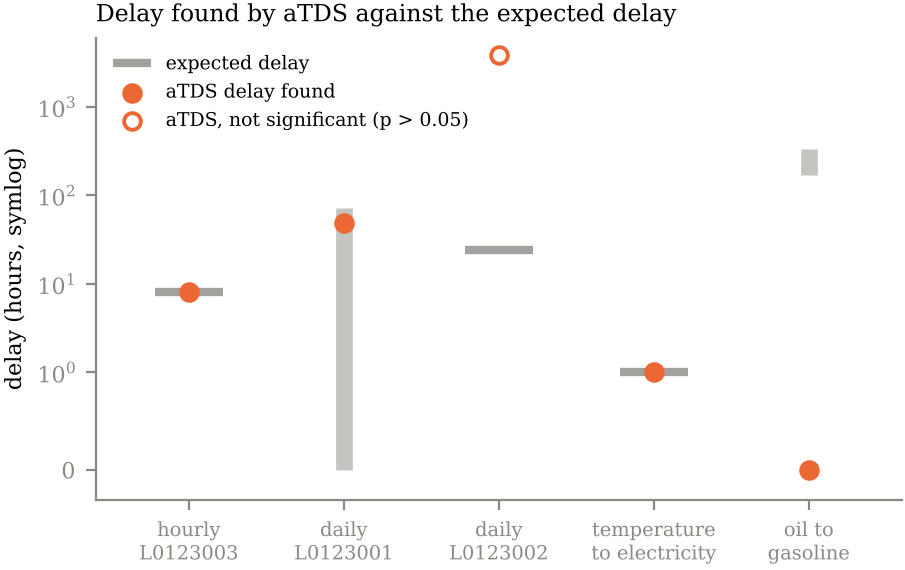
\includegraphics[width=0.6\textwidth]{figures/fig_fields_summary.png}
\caption{Delay found by aTDS (dots) against the delay expected from the domain (bars), per record. Hollow dot: not significant ($p > 0.05$).}
\label{fig:fieldssummary}
\end{figure}

\section{Summary of All Comparisons with Fixed TDS}
\label{app:scoreboard}
\Cref{tab:scoreboard} lists every comparison between aTDS and fixed TDS reported in this study, for reference. It is a catalogue, not a weighing of evidence: the rows are not independent (several share signals, pairs or settings), they differ greatly in size and importance, and many outside the design regime of fixed TDS reflect that fixed TDS was applied unchanged at a mismatched time scale. Records from other fields are excluded, since fixed TDS was not intended for them.

In the design regime of fixed TDS (1-Hz sleep data, $r = 1$), aTDS is equal in most comparisons; it is worse by a negligible AUC loss at $r = 1$ and in the wake contrast of significant links in the sleep cohort. Outside that regime, it is worse in false stability, which is higher but within budget, and in agreement with the beat-by-beat pulse arrival time; for a rhythm with a delay beyond half a period it improves detection but, like fixed TDS, reports an incorrect delay. Against rescaled fixed TDS, detection is similar, and aTDS is better in delay recovery at $r = 8$ and in the control level of the ECG cohort. On the simulated delay patterns, aTDS labels 86--90\,\% of windows stable against 6--11\,\% for fixed TDS, 99\,\% of its stable windows lie on the true delay, and its false stability in controls is 4.0--4.3\,\%, compared with under 1\,\% for fixed TDS (AUC 1.0 for both; 0.90 for fixed TDS in the on/off pattern).

\begin{table}[!htbp]
\centering
\caption{All comparisons between fixed TDS (60 / $\pm30$ / $\pm1$ samples) and aTDS, grouped by whether the data lie within the design regime of fixed TDS (1-Hz sleep data; $r = 1$). ``Better'' and ``worse'' require non-overlapping 95\,\% intervals, a paired 95\,\% interval of the difference that excludes zero, or a clear difference in counts; otherwise ``equal''. ``Rule'' rows: ``fixed TDS'' is the fixed value of the rule tested, the other two rules as in aTDS. ``Vs rescaled'' rows: rescaled fixed TDS in the fixed-TDS column; this baseline exists only for the slow-down test and the ECG cohort. The comparisons are not independent.}
\label{tab:scoreboard}
\scriptsize
\begin{tabularx}{\textwidth}{>{\raggedright\arraybackslash}p{4.1cm}>{\raggedright\arraybackslash}X>{\raggedright\arraybackslash}X>{\raggedright\arraybackslash}p{1.65cm}}
\toprule
Test & Fixed TDS & aTDS & aTDS is \\
\midrule
\multicolumn{4}{l}{\emph{Within the design regime of fixed TDS (1-Hz sleep data; $r = 1$)}} \\
Rule: tolerance, $r = 1$ (AUC change) & -- & $-0.005$ [$-0.012$, $-0.001$] & worse (tiny) \\
Slow-down, $r = 1$ (original scale) & AUC 0.997 & 0.995 & equal \\
EEG benchmark pair (delay 0) & detected (50.8\,\%), delay 0 & detected (95.5\,\%), delay 0 & equal \\
35-subject sleep cohort, stage contrasts & reproduced & reproduced, no gain & equal \\
\quad wake vs deep sleep, significant links & $d_z$ 1.16 & 0.34 (gain $-1.17$ [$-1.65$, $-0.77$]) & worse \\
\midrule
\multicolumn{4}{l}{\emph{Outside the design regime: each rule on its own (fixed value of that rule only)}} \\
Rule: window, 4$\times$ slower system & AUC 0.51 & 0.79 & better \\
Rule: lag range, delays beyond 30 samples & incorrect delay in 50 / 50 (16 opposite sign) & correct in 50 / 50 & better \\
Rule: tolerance, $r = 8$ (delay found) & 66\,\% & 85\,\% & better \\
Rule: tolerance, chance score on new data & -- & 3.3--4.4\,\% (budget 5\,\%) & as designed \\
\midrule
\multicolumn{4}{l}{\emph{Outside the design regime: simulated data}} \\
Slow-down, $r = 2$ / 4 / 8 & 0.89 / 0.59 / 0.54 & 0.98 / 0.92 / 0.88 & better \\
Slow-down, $r = 16$ & 0.51 & 0.65 (paired $+0.14$ [0.03, 0.25]) & better \\
\quad vs rescaled, $r = 2$ / 4 / 8 / 16 & 0.99 / 0.96 / 0.81 / 0.69; delay at $r = 8$: 60\,\% & 0.98 / 0.92 / 0.88 / 0.65; delay at $r = 8$: 85\,\% & equal; delay better at $r = 8$ \\
Delay patterns (5), stable windows & 6--11\,\% & 86--90\,\% & better \\
\quad stable windows on the true delay & 94--97\,\% & 99\,\% & equal \\
\quad false stability in controls & 0.7--0.9\,\% & 4.0--4.3\,\% (budget 5\,\%) & worse \\
\quad AUC & 1.00 (on/off 0.90) & 1.00 & equal \\
Long memory, $H = 0.6$ / 0.75 & 0.60 / 0.70 & 0.59 / 0.65 & equal \\
Long memory, $H = 0.9$ & 0.46 & 0.82 & better \\
Rhythm, $d = 8$ & 0.97, delay 43\,\% & 1.00, 100\,\% & better \\
Rhythm, $d = 30$ (beyond half a period) & 0.46, delay 0\,\% & 0.995, 0\,\% (detection better; delay incorrect in both) & mixed \\
Rulkov neurons, $d = 16$ / 32 & 0.73 / 0.79 & 1.00 / 1.00 & better \\
Fast signal, $d = 50$ (default) & 0.56 & 0.56 (1.00 with $d_{\max}$) & equal \\
Mixed system, slow pair & 0.44 & 0.99 & better \\
Slow $x$ drives fast $y$ & 0.83, delay 57\,\% & 1.00, 100\,\% & better \\
Changing dynamics, 2nd half & 0.71, delay 45\,\% & 0.96, 90\,\% & better \\
\midrule
\multicolumn{4}{l}{\emph{Outside the design regime: physiological data at 125\,Hz}} \\
ECG $\to$ finger pulse, 53 patients & AUC 0.69, 14 / 53 & per pair 0.95, 49 / 53; one set 0.96, 50 / 53 & better \\
\quad delay vs full-record alignment & 22 / 41 & 40 / 53 (one set: 38 / 50) & better \\
\quad delay vs pulse arrival time & 32 / 41 & 24 / 53 & worse \\
\quad vs rescaled (one set each) & AUC 0.96, 43 / 53; controls' 95th pct 39.2\,\% & AUC 0.96, 50 / 53; 1.26\,\% & equal; controls better \\
\bottomrule
\end{tabularx}
\end{table}

\paragraph{Original motivation and summary paragraphs.} The fixed parameters are expressed in samples and were chosen for 1-Hz sleep recordings. At other time scales or sampling rates, the windows contain too little information, the lag range is too narrow and the accepted fluctuation of the delay is too small. The consequence is not only reduced detection but undetected errors: a fixed lag range returned high TDS scores (72--96\,\%) with incorrect delays, some of them with the opposite sign, and fixed TDS lost nearly all detection once the system was four times slower than assumed.

\bibliographystyle{unsrtnat}
\bibliography{references}

\end{document}
